\chapter{Experiment and Result}
brief of experiment and result.
\section{Experiment}
Please tell how the experiment conducted from method.

\section{Result}
Please provide the result of experiment

\section{Imron Sumadireja/1164076}
\subsection{Teori}
\begin{enumerate}
\item Klasifikasi Teks dan Gambar Ilustrasi \par
Klasifikasi teks merupakan sebuah model yang digunakan untuk mengkategorikan teks ke dalam kelompok-kelompok yang lebih terorganisir. Jadi untuk setiap kalimat yang di masukan ke dalam mesin, mesin tersebut akan menjadikan setiap kata dari kalimat tersebut menjadi sebuah kolom. Untuk ilustrasinya bisa dilihat pada gambar berikut \ref{Teks1}
		\begin{figure}[ht]
		\centerline{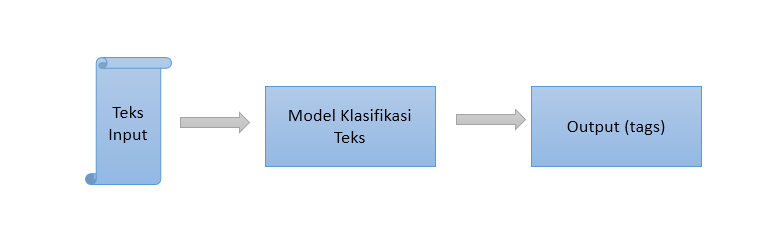
\includegraphics[width=0.5\textwidth]{figures/im/teks1.png}}
		\caption{Klasifikasi teks.}
		\label{Teks1}
		\end{figure}

\item Mengapa klasifikasi bunga tidak bisa menggunakan machine learning \par
Karena machine learning tidak dapat menampilkan inputan sesuai dengan apa yang kita inputkan. Karena inputan tersebut serupa namun mesin memberikan output yang berbeda, biasanya output atau error ini disebut dengan istilah noise. Untuk contoh sederhananya misalkan kita inputkan salah satu label yang terdapat pada bunga, output yang dihasilkan oleh mesin tersebut ialah label yang lain. Itu dikarenakan bunga banyak jenis yang serupa namun tidak sama. Untuk ilustrasinya bisa dilihat pada gambar berikut \ref{Teks2}
		\begin{figure}[ht]
		\centerline{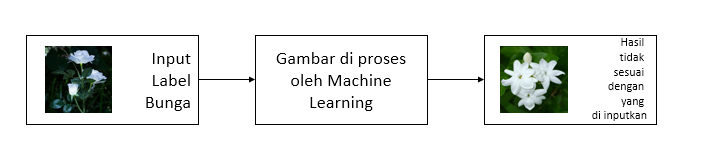
\includegraphics[width=0.5\textwidth]{figures/im/teks2.png}}
		\caption{Klasifikasi Bunga.}
		\label{Teks2}
		\end{figure}

\item Teknik pembelajaran mesin pada untuk kata-kata yang digunakan pada Youtube \par
Teknik yang digunakan pada youtube salah satunya ialah keywords. Dengan keywords tersebut mesin dapat memberikan video sesuai dengan keyword yang kita inputkan pada kolom pencarian. Teknik pembelajarannya tergantung user memberikan input teks seperti apa, karena pada youtube itu sendiri akan menyesuaikan dengan apa yang biasa kita inputkan dan akan memfilter video secara otomatis seuai dengan keyword yang biasa kita inputkan. Contoh ilustrasi sederhananya seperti berikut \ref{Teks3}
		\begin{figure}[ht]
		\centerline{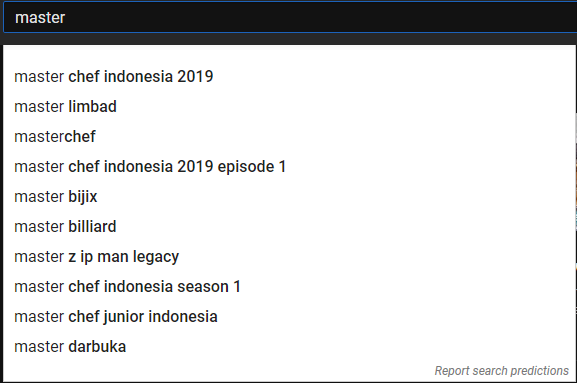
\includegraphics[width=0.5\textwidth]{figures/im/teks3.png}}
		\caption{Klasifikasi teks Youtube.}
		\label{Teks3}
		\end{figure}

\item Vektorisasi data \par
Vektorisasi data merupakan pemecahan atau pembagian data berupa teks, sebagai contoh terdapat 5 paragraf, data teks tersebut di pecah menjadi kalimat-kalimat yang lebih sederhana, lalu di pecah lagi menjadi kata untuk setiap kalimatnya. 

\item Bag of Words \par
Representasi penyederhanaan sebuah kalimat atau perhitungan setiap kata pada suatu kalimat dengan presentase berapa kali muncul kata tersebut untuk setiap kalimatnya. Contoh ilustrasi sederhananya seperti berikut \ref{Teks5}
		\begin{figure}[ht]
		\centerline{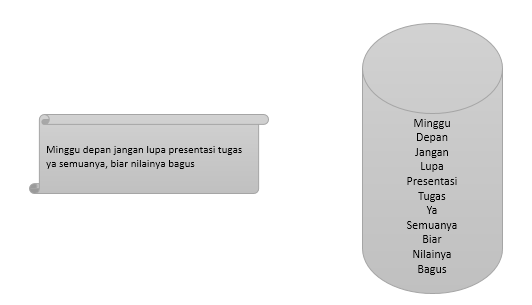
\includegraphics[width=0.5\textwidth]{figures/im/teks5.png}}
		\caption{Bag of Words.}
		\label{Teks5}
		\end{figure}

\item Apa itu TF-IDF \par
TF-IDF merupakan metode untuk menghitung bobot setiap kata pada suatu kalimat yang paling sering digunakan. TF-IDF ini akan menghitung nilai Term Frequency dan Inverse Document Frequency pada setiap kata dalam setiap kalimat yang muncul dengan diimbangi dengan jumlah dokumen dalam korpus yang mengandung kata. Contoh ilustrasi sederhananya seperti gambar berikut \ref{Teks6}
		\begin{figure}[ht]
		\centerline{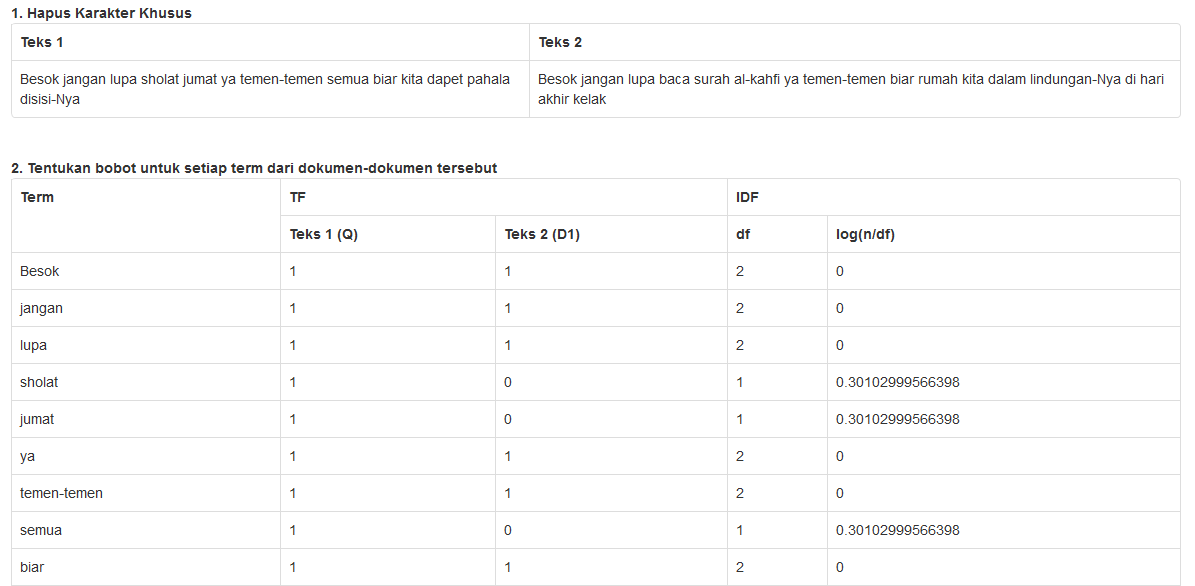
\includegraphics[width=1\textwidth]{figures/im/teks6.png}}
		\caption{TF-IDF.}
		\label{Teks6}
		\end{figure}
\end{enumerate}

\section{Yusniar Nur Syarif Sidiq/1164089}
\subsection{Teori / Yusniar Nur Syarif Sidiq / 1164089}

\begin{enumerate}
\item Jelaskan apa itu klasifikasi teks, sertakan gambar ilustrasi buatan sendiri.
Klasifikasi teks merupakan sebuah proses pemberian tag atau kategori kedalam teks sesuai dengan isinya. Fungsi dari klasifikasi teks yaitu untuk melakukan klasifikasi atau pengelompokkan teks ke dalam sebuah label tertentu. Untuk contoh klasifikasi teks dapat dilihat pada figure \ref{YNC4-1}

	\begin{figure}[ht]
		\centering{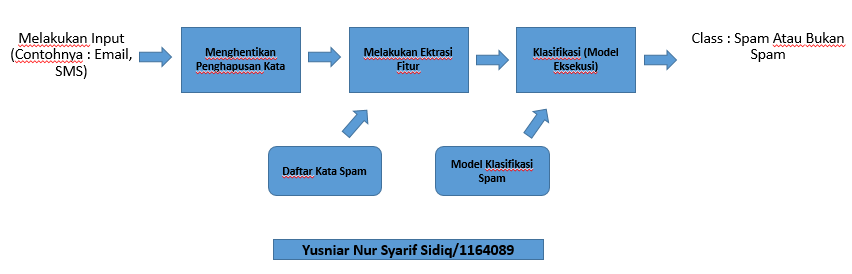
\includegraphics[scale=0.5]{figures/YN/Chapter4/YNC4-1.png}}
		\caption{Contoh Klasifikasi Teks YN}
		\label{YNC4-1}
	\end{figure}

Dimana dalam figure \ref{YNC4-1} menjelaskan terdapat daftar kata berupa kata-kata yang cukup banyak muncul pada email anda dengan tujuan menawarkan sesuatu barang atau hal lainnya, maka dapat dikategorikan bahwa kata tersebut merupakan spam.

\item Jelaskan mengapa klarifikasi bunga tidak bisa menggunakan machine learning, sertakan ilustrasi sendiri.
Karena semua bunga belum tentu memiliki ciri-ciri yang sama, atau bisa dibilang adanya data noise dalam klasifikasi bunga yang dapat menyebabkan tidak bisa menggunakan Machine Learning. Akan saya beri contoh berdasarkan ilustrasi saya sendiri, terdapat bunga mawar bewarna merah yang memiliki jumlah 5 kelopak, lalu terdapat bunga selain mawar yang  berwarna merah dan memiliki jumlah kelopak yang sama yaitu 5 serta memiliki kategori yang cukup banyak. Lalu terdapat bunga yang tidak cukup jelas datanya baik warnanya maupun jumlah kelopaknya, data tersebut akan menyababkan data noise. Untuk ilustrasi gambar akan saya berikan 2 buah gambar bunga dengan warna yang sama akan tetapi jenis yang berbeda, dapat dilihat pada figure \ref{YNC4-2}

	\begin{figure}[ht]
		\centering{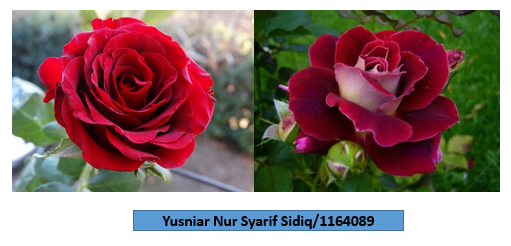
\includegraphics[scale=0.5]{figures/YN/Chapter4/YNC4-2.png}}
		\caption{Contoh Klasifikasi Bunga YN}
		\label{YNC4-2}
	\end{figure}

\item Jelaskan bagaimana teknik pembelajaran mesin pada teks pada kata-kata yang digunakan di youtube
Dapat menggunakan teknik bag-of-words pada klasifikasi berbasis text dan kata guna mengklasifikasikan sebuah komentar yang ada dalam internet sebagai kata spam atau bukan. Contohnya pada kolom komentar dapat di cek seberapa sering kata yang muncul dalam kalimat. Setiap kata bisa disebut sebagai baris dan kolomnya, hal ini merupakan dimana kategori kata spam atau tidak. Untuk ilustrasi gambarnya dapat dilihat pada figure \ref{YNC4-3}

	\begin{figure}[ht]
		\centering{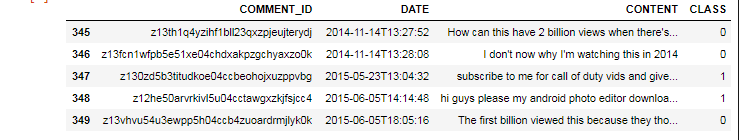
\includegraphics[scale=0.5]{figures/YN/Chapter4/YNC4-3.png}}
		\caption{Teknik Pembelajaran Mesi Pada Teks Youtube YN}
		\label{YNC4-3}
	\end{figure}


\item Jelaskan apa yang dimaksud vektorisasi data.
Vektorisasi data merupakan pembagian dan pemecahan data lalu data tersebut akan dilakukan perhitungan. Vektorisasi dapat kita maksudkan setiap data yang mungkin kita petakan ke integer tertentu. Misalnya saja kita memiliki data array yang cukup besar maka setiap kata cocok dengan slot unik dalam array. Contoh kita memiliki banyak kata yang tersesun dengan beberapa paragraf, data tersebut nantinya akan kita pecah mejadi bebera kata dalam tiap kalimatnya.

\item Jelaskan apa itu bag of words dengan kata-kata yang sederhana dan ilustrasi sendiri
bag-of-words adalah representasi penyederhanaan yang digunakan dalam pemrosesan bahasa alami dan pengambilan informasi. Model bag-of-words sederhana untuk dipahami dan diterapkan dan telah melihat kesuksesan besar dalam masalah seperti pemodelan bahasa dan klasikasi dokumen. Ilustrasinya yaitu terdapat satu kalimat dan kalimat tersebut akan dipecah menjadi kata per kata, untuk lebih jelasnya dapat dilihat pada figure \ref{YNC4-4}

	\begin{figure}[ht]
		\centering{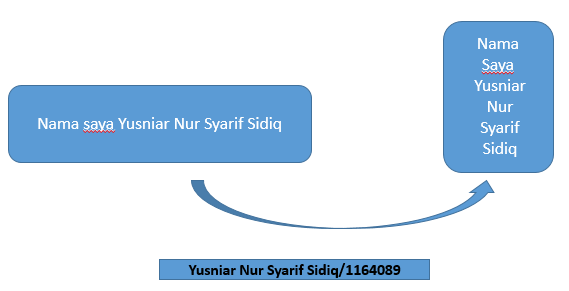
\includegraphics[scale=0.5]{figures/YN/Chapter4/YNC4-4.png}}
		\caption{Bag Of Words YN}
		\label{YNC4-4}
	\end{figure}

\item Jelaskan apa itu TF-IDF, ilustrasikan dengan gambar sendiri
TF-IDF dapat memberikan kita frekuensi kata dalam setiap dokumen sehingga dapat menggantikan data menjadi number. TD-IDF merupakan sebuah metode untuk dapat menghitung bobot setiap kata dalam kalimat yang sering digunakan. Untuk lebih jelasnya dapat dilihat dari figure \ref{TNC4-5}

	\begin{figure}[ht]
		\centering{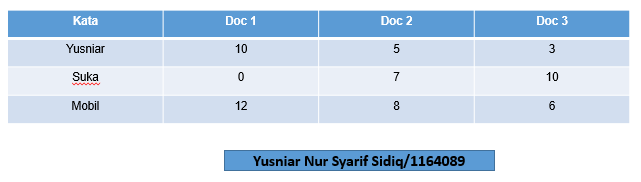
\includegraphics[scale=0.5]{figures/YN/Chapter4/YNC4-5.png}}
		\caption{TF-IDF YN}
		\label{YNC4-5}
	\end{figure}


\end{enumerate}